\documentclass[letterpaper,onecolumn,10pt,journal,final]{IEEEtran}

\usepackage{latexsym}


\usepackage[spanish,es-tabla]{babel}

\usepackage{amsfonts}
\usepackage{subfigure}
\usepackage{psfrag}
\usepackage{colortbl}
\usepackage{color}
\usepackage[sectionbib]{chapterbib}
\usepackage{afterpage}
\usepackage{booktabs}


\usepackage{graphicx}
\usepackage{url}
\usepackage{amsmath}
\interdisplaylinepenalty=2500
\usepackage[english]{babel}
%\usepackage{array,booktabs,arydshln,xcolor}
\usepackage{flushend}
\hyphenation{industrial electronics IEEEtran}
\usepackage[font=footnotesize,caption=false,farskip=0mm,captionskip=0mm,nearskip=0mm]{subfig}
\usepackage{cite}
\usepackage{amsmath}
\usepackage{array}
\usepackage{graphicx}
\usepackage{latexsym}
\usepackage{psfrag}
\usepackage{color}
\usepackage{multirow}
\usepackage{stfloats}
\usepackage{enumerate}
% Paquetes adicionales para insertar código con formato m-file de MATLAB
\usepackage{listings}   % Permite incorporar código con diferentes formatos
\usepackage{float}
%usepackage{caption}
\usepackage[font=bf]{caption}
% falta cambiar el font size de caption  a 9pt
\usepackage[dvips]{graphicx}
\usepackage[framed,numbered,final]{mcode}% Configura listings para que el resultado se vea igual al editor de MATLAB
\usepackage{xcolor}
\usepackage{textcomp}

%\usepackage [latin1]{inputenc}
%\renewcommand\lstlistingname{Code}% Cambia el nombre del objeto listings

%ejemplo matlab code:

%\begin{lstlisting}[frame=single]
%a = 15;				% Por defecto es tipo 'double'
%b = uint8(a);		
%c = int16(32767);
%\end{lstlisting}

\parskip 0pt

\usepackage{lipsum}

\newcommand\blfootnote[1]{%
  \begingroup
  \renewcommand\thefootnote{}\footnote{#1}%
  \addtocounter{footnote}{-1}%
  \endgroup
}

\begin{document}
\title{ELO 314 - Procesamiento Digital de Señales\\ Laboratorio 1: Señales Discretas en MatLab}

\author{\textbf{Preparado por}
\vspace{1 mm}Juan Aguilera e-mail: Juan.Aguileraca@sansano.usm.cl \\
            Cristóbal Huidobro e-mail: 
cristobal.huidobro@sansano.usm.cl}

\maketitle

\vspace{-1 cm}

%\setcounter{section}{0}
%%%%%%%%%%%%%%%%%%%%%%%%%%%%%%%%%%%%%%%%%%%%%%%%%%%%%%%%%%%%%%%%%%%%%%%%%%%%%%%%%%%%%%%%%%%%%%%%%%
%
%---------------------Representación Gráfica de señales sinusoidales----------------------------%
%
%%%%%%%%%%%%%%%%%%%%%%%%%%%%%%%%%%%%%%%%%%%%%%%%%%%%%%%%%%%%%%%%%%%%%%%%%%%%%%%%%%%%%%%%%%%%%%%%%%
\section{Representación Gráfica de señales sinusoidales}

\begin{enumerate}[{1)}]
    \item Se genera una señal con 5 veces menos muestras al aumentando el tiempo en el que se toma cada muestra en 5 veces, por lo que modificamos la variable $t$ de la siguiente manera:
    \begin{lstlisting}[frame=single]
        t = 0:10:59;
        y = sin(t/6)
    \end{lstlisting}
    Notamos que el tiempo de muestreo original es de $Ts=2~s$ y el nuevo tiempo de muestreo es $Ts = 10~s$.
    En la Figura \ref{I1} se muestran las señales resultantes al ser muestreadas con dichos tiempos usando $Stem$ y $Plot$.
    
    \begin{figure}[H]
    \centering
    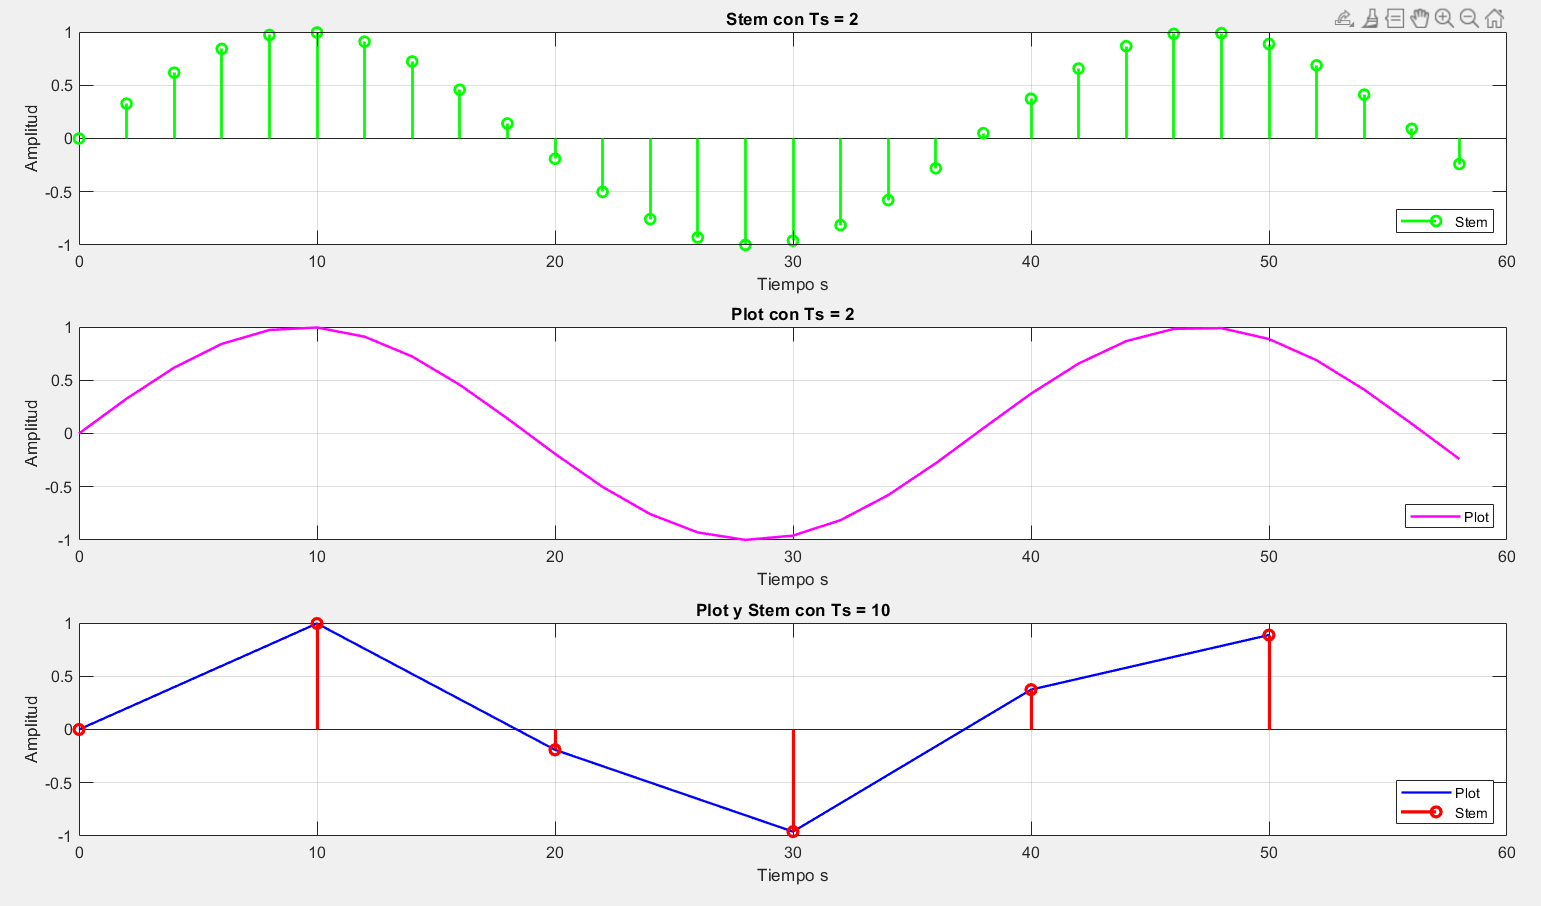
\includegraphics[scale=0.5]{Figuras/plotI1.png}
    \caption{Gráficos usando Stem y Plot para Ts = 2 y Ts = 10.}\label{I1}
    \end{figure}
    
    \item El comando $stem()$  muestra los valores discretos que fueron tomados de la señal, el comando $Plot$ trata de hacer una aproximación de los valores continuos de la señal, conectando linealmente los valores en los puntos de muestreo. Estas comparaciones se aprecian en la Figura \ref{I1}.
    \item Como muestra el comando $stem()$ en el ultimo gráfico de la Figura \ref{I1}, la cantidad de valores discretos de la señal resultante se reduce 5 veces.
    \item El intervalo [0 59] representa el tiempo en segundos.
    \item Las señales tienen una duración de 59 segundos. Las señales tienen un periodo aproximado de $12\pi~s \approx 38~s$ al igual que la señal original y por lo tanto una frecuencia de $0.0265~Hz$. %Se observa que 
    \item $stairs()$ grafica el valor de una muestra continuamente hasta la siguiente como se muestra en la Figura \ref{I6}. Este comando es útil si se quiere graficar un sistema que implementa un retentor de orden 0.
    
    \begin{figure}[H]
    \centering
    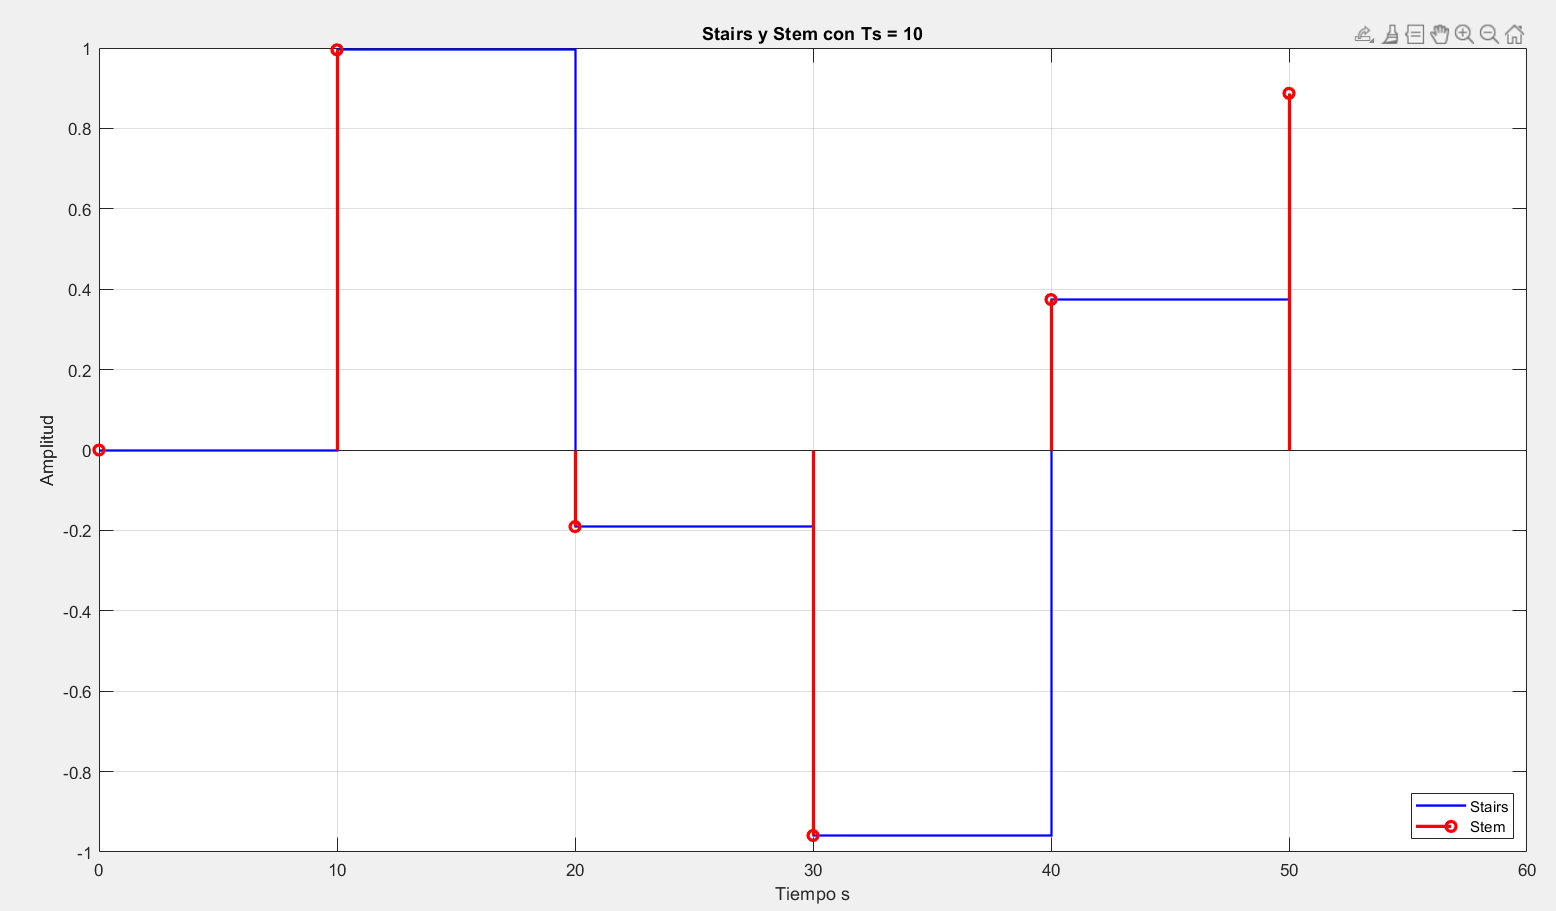
\includegraphics[scale=0.4]{Figuras/plotI6.png}
    \caption{Gráfico usando Stairs y Stem para Ts = 10.}\label{I6}
    \end{figure}
    
    En la Figura \ref{I6} notamos que $stairs()$ comienza junto a la muestra inicial en cero con $stem()$, luego sigue con un valor constante hasta la siguiente muestra.
    
    
\end{enumerate}

%%%%%%%%%%%%%%%%%%%%%%%%%%%%%%%%%%%%%%%%%%%%%%%%%%%%%%%%%%%%%%%%%%%%%%%%%%%%%%%%%%%%%%%%%%%%%%%%%%
%
%------------------------------------MUESTREO----------------------------------------------------%
%
%%%%%%%%%%%%%%%%%%%%%%%%%%%%%%%%%%%%%%%%%%%%%%%%%%%%%%%%%%%%%%%%%%%%%%%%%%%%%%%%%%%%%%%%%%%%%%%%%%
\section{Muestreo}

En la Figura \ref{II1} se presentan los gráficos de la señal $s_i[n]$ con los tiempos de muestreo indicados.

\begin{figure}[H]
    \centering
    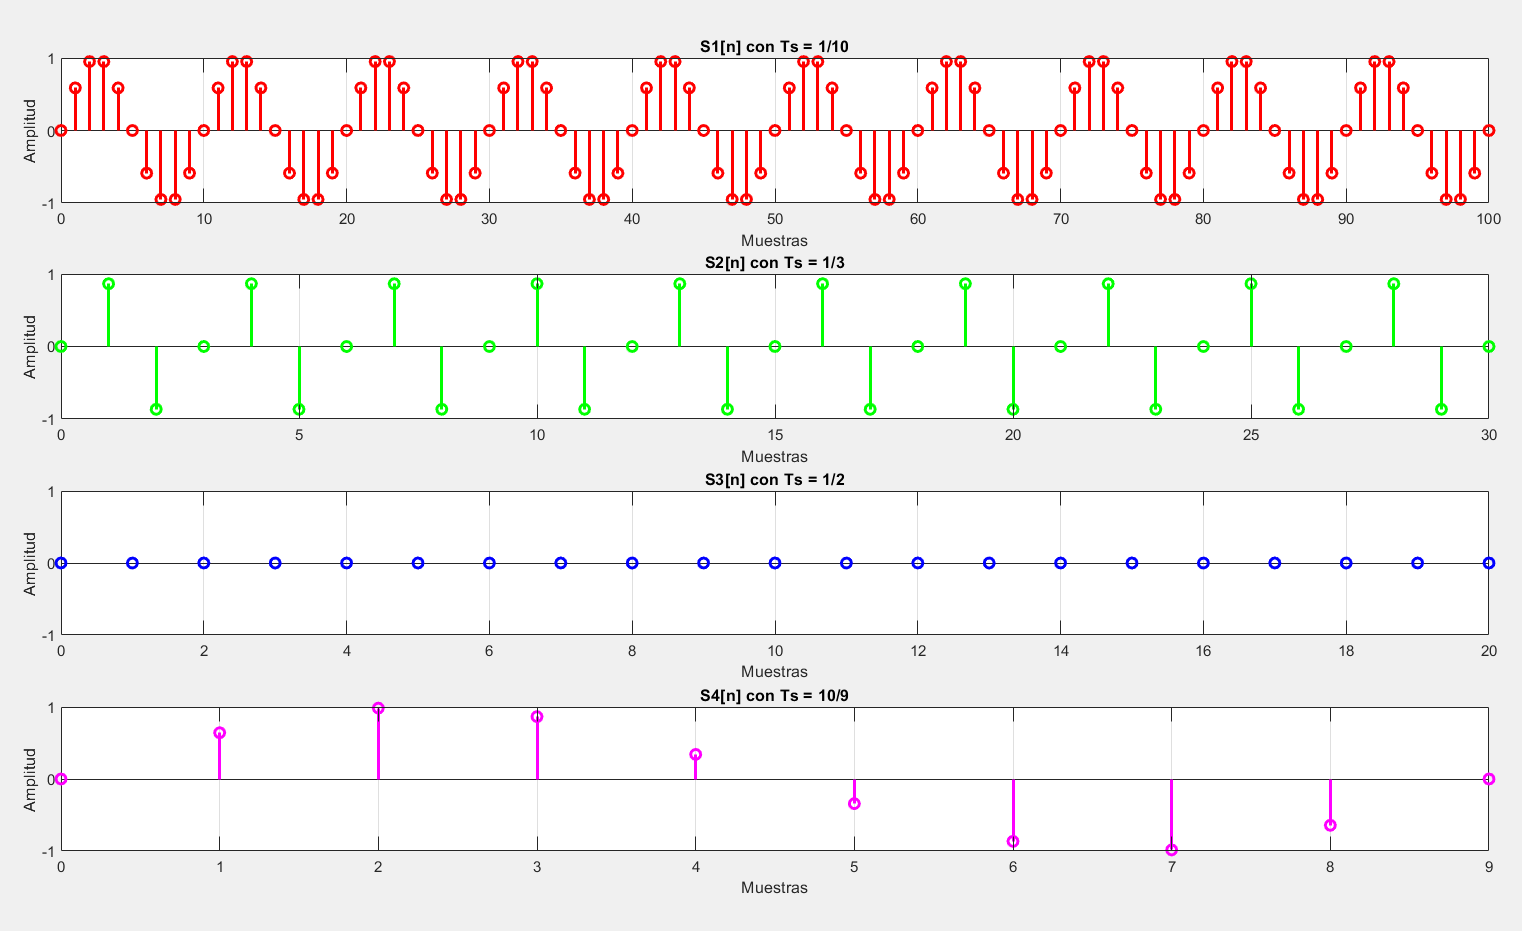
\includegraphics[scale=0.5]{Figuras/plotII1.png}
    \caption{Gráficos usando Stem para $s_i [n]$}\label{II1}
\end{figure}

\begin{enumerate}[{1)}]
    \setcounter{enumi}{4}
    \item Las frecuencias para las señales son de $1Hz$, $1Hz$, $0Hz$ y $1/10Hz$ para $s_1[n], .. ~ ,s_4[n]$ respectivamente.
    \item Se obtienen $10$, $3$, $2$ y $1$ muestras por períodos para $s_1[n], .. ~ ,s_4[n]$ respectivamente.
    \item No, las señales resultantes con un $fs$ inferior al doble de la frecuencia de la señal original ( $1~Hz$ ) se alteran por aliasing, como es el caso de la señal $s_4[n]$. cabe notar que la frecuencia obtenida en este caso es la resta de la frecuencia original con la frecuencia de sampleo.
    Además en el caso de la señal $s_3[n]$, donde $f_s = f_n$, se muestrea exactamente en los valores nulos de la señal original, obteniendo una señal nula.
    \item Las frecuencias de muestreo son de $10Hz$, $3Hz$, $2Hz$, $9/10Hz$ para $s_1[n], .. ~ ,s_4[n]$ respectivamente.
    \item si la frecuencia de muestreo de la señal esta bajo la frecuencia de Nyquist, se generan nuevas frecuencias inferiores a la frecuencia de Nyquist, este fenómeno se llama aliasing.
\end{enumerate}

%%%%%%%%%%%%%%%%%%%%%%%%%%%%%%%%%%%%%%%%%%%%%%%%%%%%%%%%%%%%%%%%%%%%%%%%%%%%%%%%%%%%%%%%%%%%%%%%%%
%
%------------------------------------Generación de señales---------------------------------------%
%
%%%%%%%%%%%%%%%%%%%%%%%%%%%%%%%%%%%%%%%%%%%%%%%%%%%%%%%%%%%%%%%%%%%%%%%%%%%%%%%%%%%%%%%%%%%%%%%%%%
\section{Generación de señales}

\begin{enumerate}[{1)}]
    \item Para muestrear la señal se eligio una frecuencia de muestreo de $5000~Hz$ ya que de esta forma respetamos el criterio de Nyquist, haciendo la $Fs$ más del doble que la mayor frecuencia $f_0$ entre las señales a muestrear. Las señales resultantes se muestran en la Figura \ref{III1}.
    \begin{figure}[H]
    \centering
    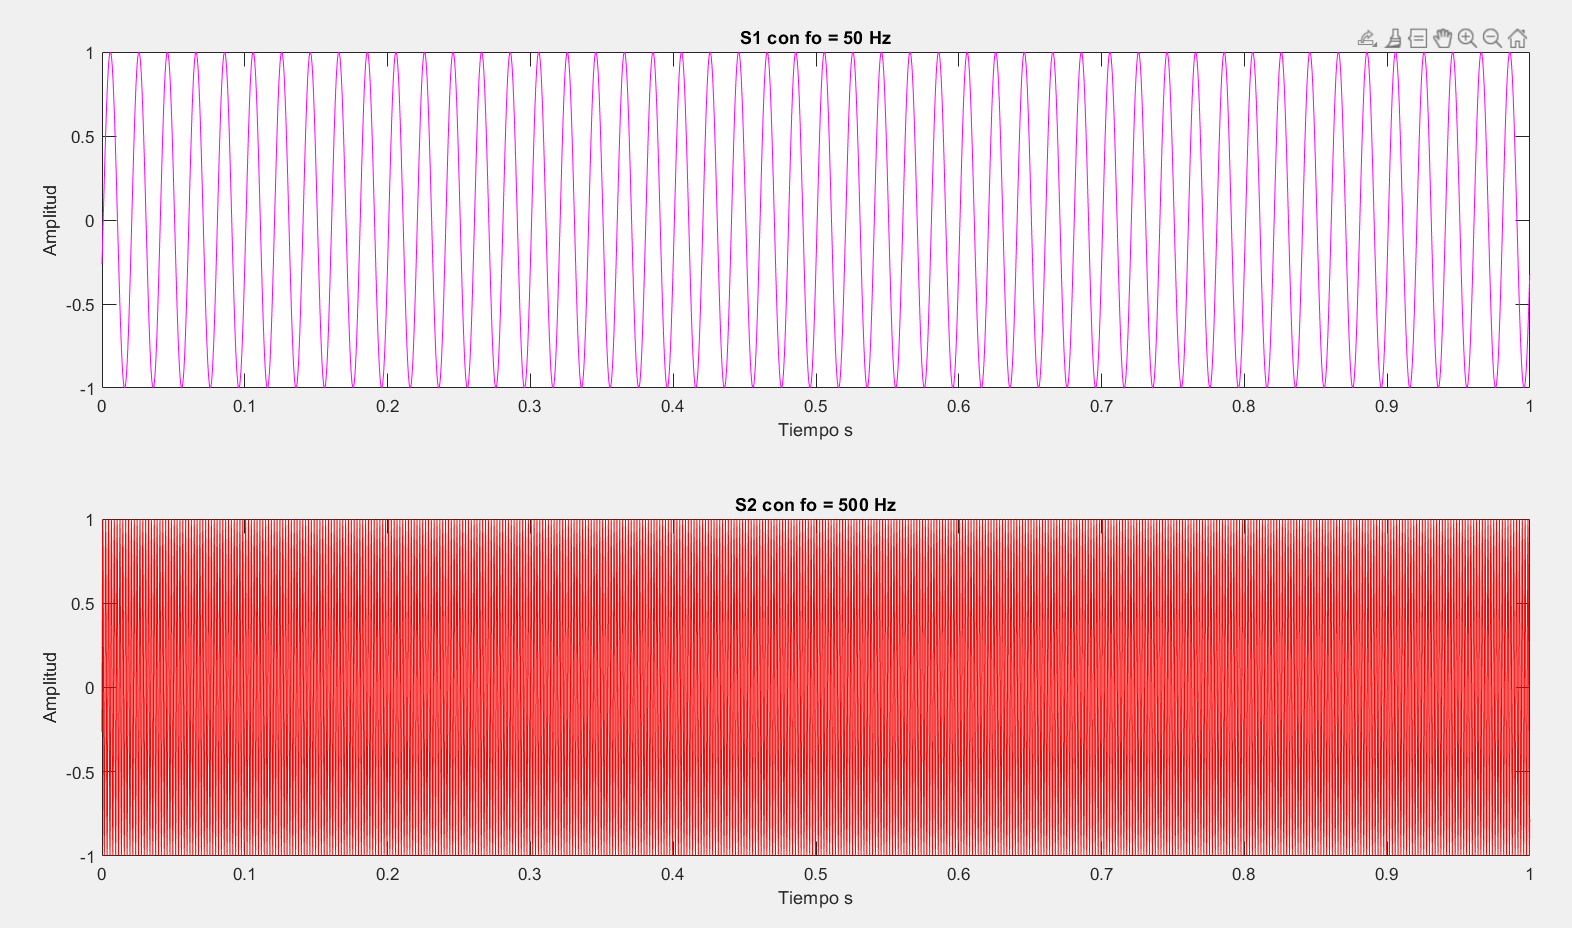
\includegraphics[scale=0.5]{Figuras/plotIII1.png}
    \caption{Plots de $s_1$ y $s_2$}\label{III1}
    \end{figure}
    se logra verificar que al multiplicar $t_{max} \cdot f_s$ obtenemos el largo del vector de la señal resultante, correspondiente a $5000$ elementos.
    \item El periodo de la señal es de $0.02~s$ como se ve en la Figura \ref{III2}, ya que un período de S1 ($0.02~s$) corresponde a 10 períodos de S2, lo que genera que ese sea el primer punto donde ambas señales completen un período.
    
    Para el caso con tonos de $300~Hz$ y $200~Hz$, el período es de $0.01~s$. Esto se debe a que el mínimo común múltiplo de los periodos (es decir, el primer punto en el que coinciden) está dado por $0.01~s$. Esto también se puede calcular por las frecuencias de las señales, donde se obtiene el máximo común divisor entre las frecuencias para encontrar la fundamental a la cual pertenecen ambos armónicos.  \\
    Para ambos casos se escuchan dos tonos puros superpuestos.\\
    
    Para la frecuencia fundamental de las señales sumadas del acorde $La-\#Do-Mi$, procedemos a obtener su mínimo común divisor, igual a $220~Hz$. Por lo tanto, las frecuencias de $880~Hz$, $1100~Hz$ y $1320~Hz$ corresponden al $4^{to}$, $5^{to}$ y $6^{to}$ armónico respectivamente.  \\
    La frecuencia fundamental corresponde a la nota $La$.
    \begin{figure}[H]
    \centering
    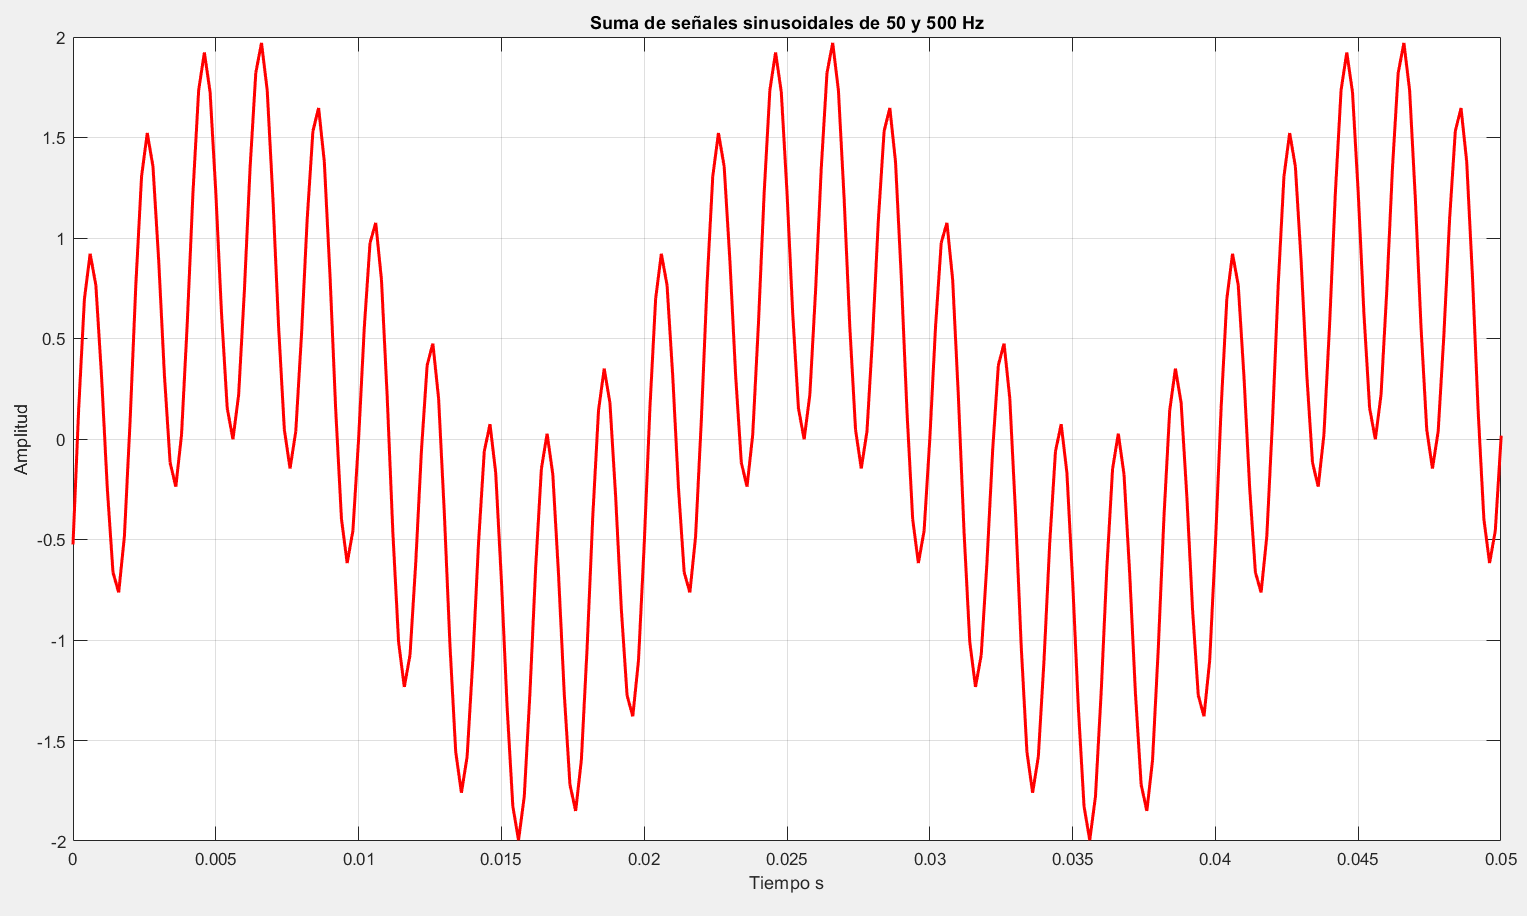
\includegraphics[scale=0.4]{Figuras/plotIII2.png}
    \caption{Suma de $s_1$ y $s_2$.}\label{III2}
    \end{figure}

    \item 
    Se utilizó el siguiente script para sintetizar la aproximación de una señal cuadrada:
    \begin{lstlisting}
    t = 0:1/100000:1;
    ss = zeros(1,100001);
    for k = 1:6
        ss = ss+sin(2*pi*(2*k-1)*220*t)/(2*k-1);
    end
    \end{lstlisting}
    En la figura \ref{fig:III3} se puede corroborar que la señal obtenida se asemeja a una señal cuadrada, con una amplitud similar a $\pi/4$.
    Al escuchar la señal, se observa que se identifica solamente una frecuencia (la fundamental, que corresponde a la frecuencia de la señal cuadrada), a pesar de que la señal generada esté formada de diversos armónicos. 
    \begin{figure}[H]
        \centering
        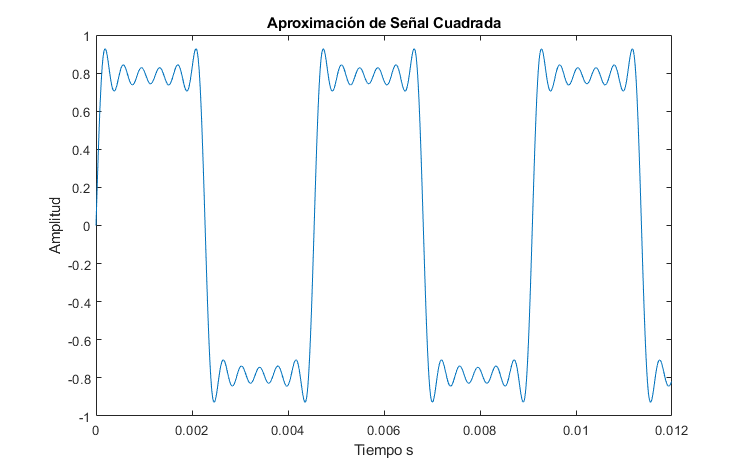
\includegraphics[width=0.7 \linewidth]{Figuras/PlotIIIc.png}
        \caption{Aproximación con 6 armónicos de señal cuadrada}
        \label{fig:III3}
    \end{figure}
    Luego, se procede a agregar un componente aleatorio con distribución uniforme a cada armónico de la señal, de modo que el comando dentro del ciclo for quede de la forma:
    \begin{lstlisting}
    ss = ss+sin(2*pi*(2*k-1)*220*t+2*pi*rand(1,1))/(2*k-1);
    \end{lstlisting}
    En la figura \ref{fig:III32} se observan las señales generadas al repetir el script varias veces. Nótese como la forma de onda cambia manteniendo la periodicidad de la señal. 
    
    Al reproducir las señales producidas corriendo el programa varias veces, se observa que si bien se sigue escuchando una misma nota musical, el timbre de ésta cambia cada vez, probando que aunque varias señales presente los mismos armónicos en igual amplitud, si la fase de ellos cambia el sonido no será el mismo.
    \begin{figure}[H]
        \centering
        \includegraphics[width=0.9 \linewidth]{Figuras/PlotIIIc2.png}
        \caption{Señal con armónicos de fase aleatoria}
        \label{fig:III32}
    \end{figure}
    \item
    Se generó una señal aleatoria con distribución uniforme entre $-1$ y $1$ y se le sumó a la señal sinusoidal de $500~Hz$ generada anteriormente. El resultado de lo anterior, junto a la señal original, se observa en los primeros dos gráficos de la figura \ref{III4}.
    
    Se observa que la forma de la señal sinusoidal se pierde al agregar esta señal aleatoria. Sin embargo, al incrementar la frecuencia de muestreo y agregar una señal aleatoria, se observa que la señal se asemeja a una sinusoidal con un ruido uniforme de amplitud $1$. Como lo muestra el tercer gráfico de la figura \ref{III4}. Esto se debe a que el comando \texttt{rand} genera una señal aleatoria distribuida uniformemente, por lo que con suficientes muestras se generarían señales que rodeen a la sinusoidal en todo el rango $[-1,1]$.
    \begin{lstlisting}
    s2 = sin(2*pi*500*t + 50); 
    random = 2*rand(1,100000)-1;
    s2_rand = s2+random;
    \end{lstlisting}
    \begin{figure}[H]
        \centering
        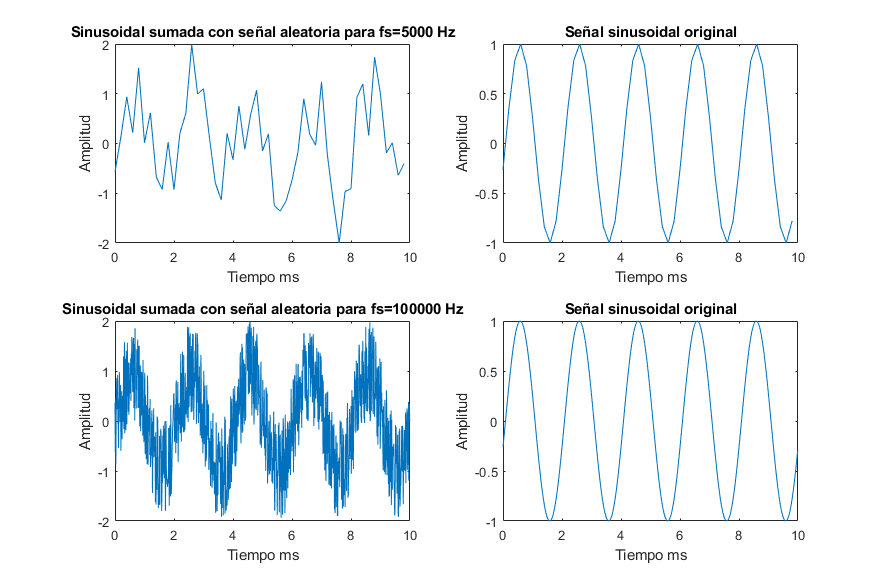
\includegraphics[width=0.85 \linewidth]{Figuras/plotIIId.png}
        \caption{Señal original y señal sumada a señal aleatoria con distintas frecuencias de muestreo}
        \label{III4}
    \end{figure}
    \item
    Se modifica el script para multiplicar la señal por una señal aleatoria entre $0.5$ y $1$. El gráfico de esta se puede observar en la figura \ref{III5}. Se aprecia el efecto de una sinusoidal escalada.
    \begin{lstlisting}
    sx_var_amp = sx.*(rand(1,0.5*fs)*0.5+0.5);
    \end{lstlisting}
    \begin{figure}[H]
        \centering
        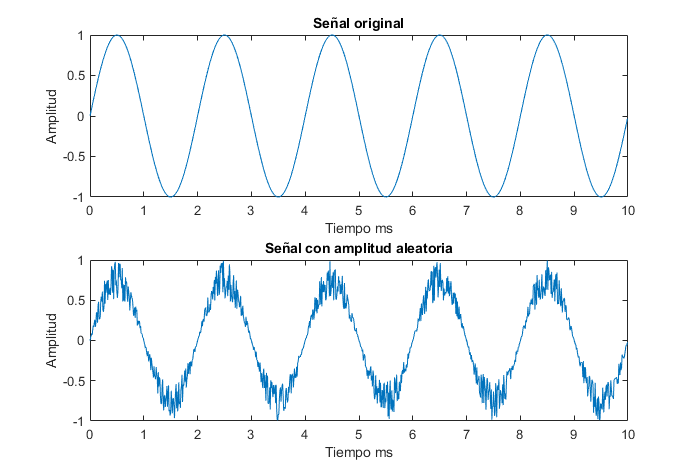
\includegraphics[width=0.7 \linewidth]{Figuras/plotIIIe.png}
        \caption{Señal sinusoidal con amplitud que varía aleatoriamente}
        \label{III5}
    \end{figure}
    \item
    Finalmente se modifica el script para sumarle una señal aleatoria entre $-\pi/2$ y $\pi/2$ a la sinusoidal, y se grafica la señal en la figura \ref{III6}. En este caso se observa que la sinusoidal se desplaza verticalmente en lugar de horizontalmente. (lo que explica la ilusión de recorte en la amplitud de esta).
    \begin{lstlisting}
    sx_var_fas = sin(2*pi*500*t2 + pi*(rand(1,fs+1)-0.5));
    \end{lstlisting}
    \begin{figure}
        \centering
        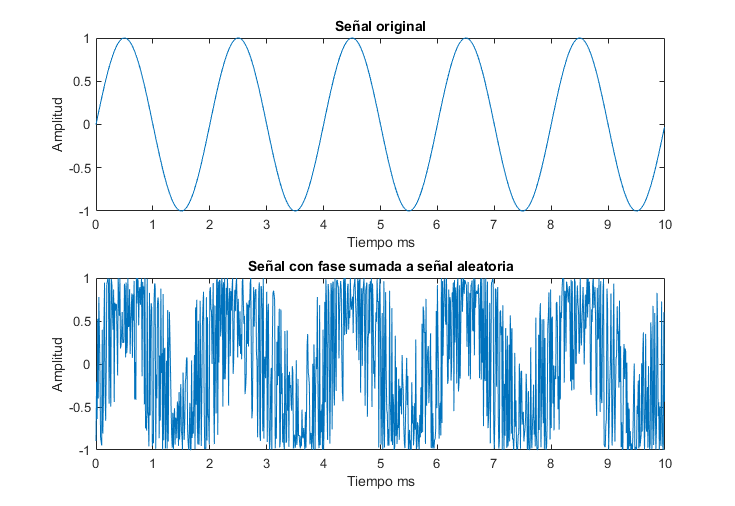
\includegraphics[width=0.7 \linewidth]{Figuras/plotIIIf.png}
        \caption{Señal sinusoidal con fase sumada a señal aleatoria}
        \label{III6}
    \end{figure}
    \item
    Como se mencionó en los puntos anteriores, al sumarle la señal aleatoria, se genera una sinusoidal que se desplaza verticalmente con $1$ de amplitud (generando el efecto visual de una sinusoidal mas ancha). Al multiplicar por la señal aleatoria se genera una sinusoidal cuya amplitud varía constantemente entre 0.5 y 1. Al agregar fase aleatoria, la señal se desplaza horizontalmente en $0.5~ms$ para cada lado.
    
    Al escuchar las señales generadas se observa que se distingue el tono inicial pero con constante ruido de fondo. El ruido escuchado es muy prominente en las señales con fase aleatoria y con ruido sumado, siendo más leve en la señal con amplitud aleatoria.
    
\end{enumerate}

%%%%%%%%%%%%%%%%%%%%%%%%%%%%%%%%%%%%%%%%%%%%%%%%%%%%%%%%%%%%%%%%%%%%%%%%%%%%%%%%%%%%%%%%%%%%%%%%%%
%
%------------------------------------Experimentando doblaje--------------------------------------%
%
%%%%%%%%%%%%%%%%%%%%%%%%%%%%%%%%%%%%%%%%%%%%%%%%%%%%%%%%%%%%%%%%%%%%%%%%%%%%%%%%%%%%%%%%%%%%%%%%%%
\section{Experimentando doblaje}

\begin{enumerate}[{1)}]
    \item 
    Luego del downsampling, las señales se escuchan en un principio igual a la original, pero luego de cierto punto la frecuencia empieza a disminuir en lugar de seguir aumentando. Esto se debe a que las nuevas frecuencias de sampleo son menores al doble de la frecuencia de Nyquist, por lo que la señal original contiene frecuencias superiores a las permitidas por la tasa de muestreo. éstas son reflejadas en la creación de nuevas frecuencias menores a la de Nyquist en el sistema, provocándose el femómeno del $aliasing$.
    \item Para evitar el efecto del $aliasing$ es necesario respetar la frecuencia de Nyquist al re-muestrear la señal, por lo tanto buscamos la máxima frecuencia de la señal, lo que se aprecia en la Figura \ref{IV2} cercano a $5~kHz$ por lo que la mínima frecuencia de muestreo seria $f_{s~min} = 10~kHz$.
    \begin{figure}[H]
    \centering
    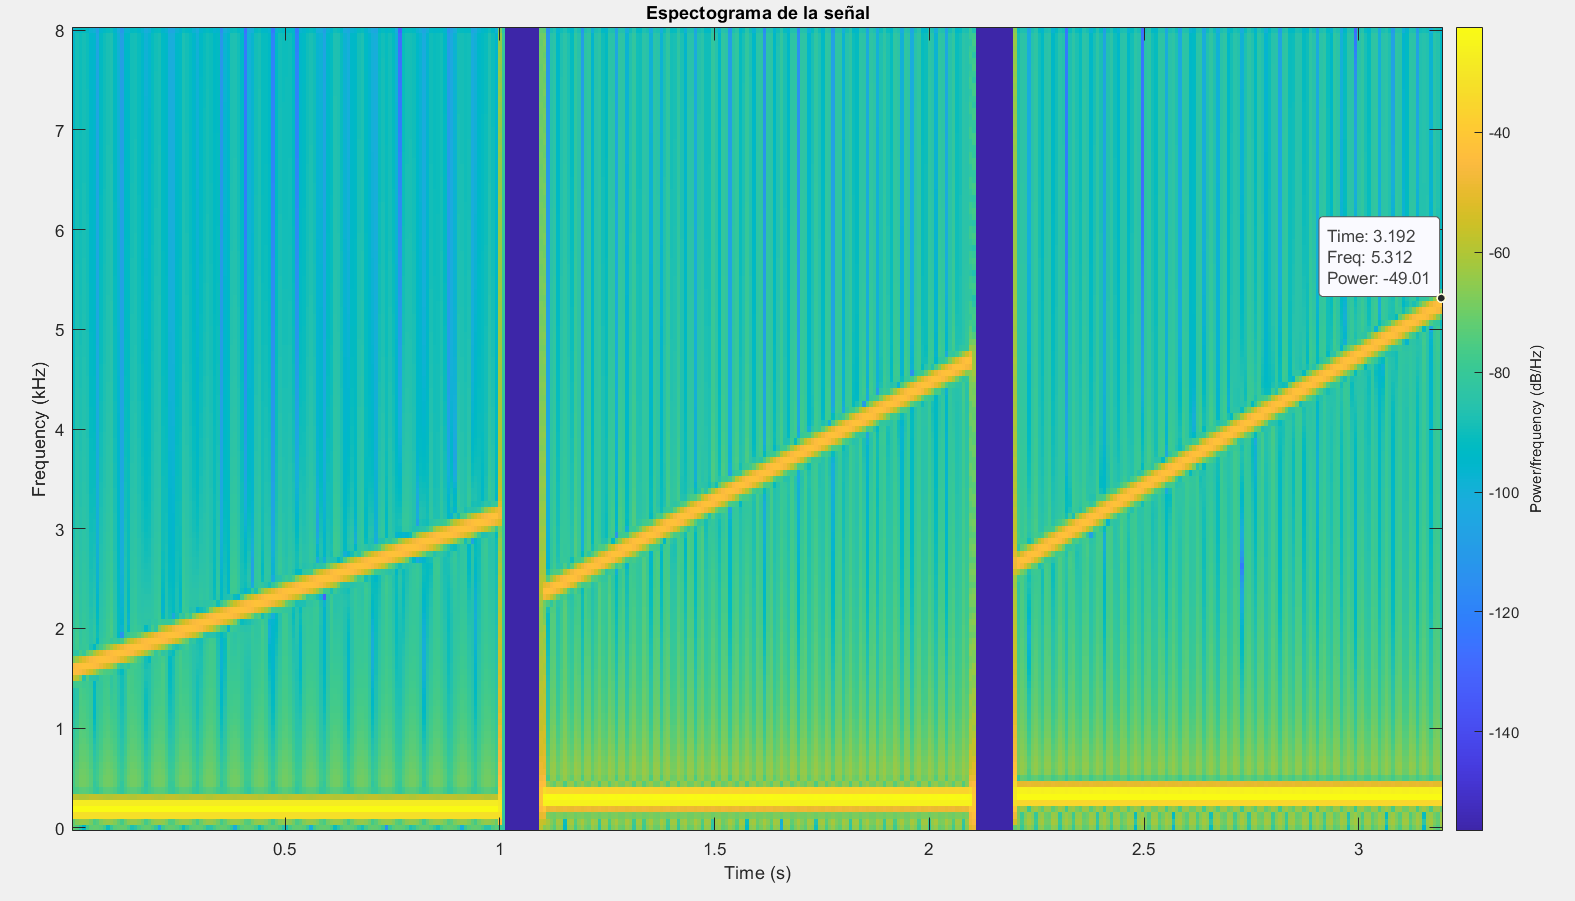
\includegraphics[scale=0.4]{Figuras/plotIV2.png}
    \caption{Espectrograma de aliasing\_test.}\label{IV2}
    \end{figure}
\end{enumerate}

%%%%%%%%%%%%%%%%%%%%%%%%%%%%%%%%%%%%%%%%%%%%%%%%%%%%%%%%%%%%%%%%%%%%%%%%%%%%%%%%%%%%%%%%%%%%%%%%%%
%
%---------------------EFECTOS DE LA CUANTIZACI ́ON EN PROCESADORES DIGITALES----------------------%
%
%%%%%%%%%%%%%%%%%%%%%%%%%%%%%%%%%%%%%%%%%%%%%%%%%%%%%%%%%%%%%%%%%%%%%%%%%%%%%%%%%%%%%%%%%%%%%%%%%%
\section{Efectos de la cuantización en procesadores digitales}

\begin{enumerate}[{1)}]
    \item La función implementada se muestra a continuación:
    
    \begin{lstlisting}[frame=single]
    function c = cuantiza(x,N)
    delta = (max(x)-min(x))/(N-1);
    S1 =  (x-min(x))/delta;
    c = round(S1);
    end
    \end{lstlisting}
    
    Al reproducir las señales cuantizadas para 12 y 8 bits no se perciben diferencias con la señal original, pero si una leve disminución en el volumen. A partir de los 4 bits se distingue ruido en la señal cuantizada, este efecto aumentan con 2 y 1 bits de cuantización donde además se percibe un mayor volumen que en la señal original, debido a los pocos niveles de cuantización.\\

    El audio que más se deteriora es $musica\_16\_16.wav$. Esto se podría explicar por que la que la señal de voz en general esté mejor distribuída respecto a su amplitud máxima, por lo que aprovecharía mejor la totalidad de los niveles de cuantización.

    
    
    \item
    \begin{enumerate}[{a)}]
        \item 
        
        El código usado para la función \texttt{[y,e] = cuantiza2(x,N)} es el siguiente
        \begin{lstlisting}
        function [y, e] = cuantiza2(x,N)
            delta = (max(x)-min(x))/(N-1);
            S1 =  (x-min(x))/delta;
            S11 = round(S1);
            y = S11.*delta + min(x);
            e = y - x;
        end 
        \end{lstlisting}
        
        El gráfico de las señales cuantizadas sobre la señal original se muestra en la Figura \ref{V2a} a continuación.
        
        \begin{figure}[H]
        \centering
        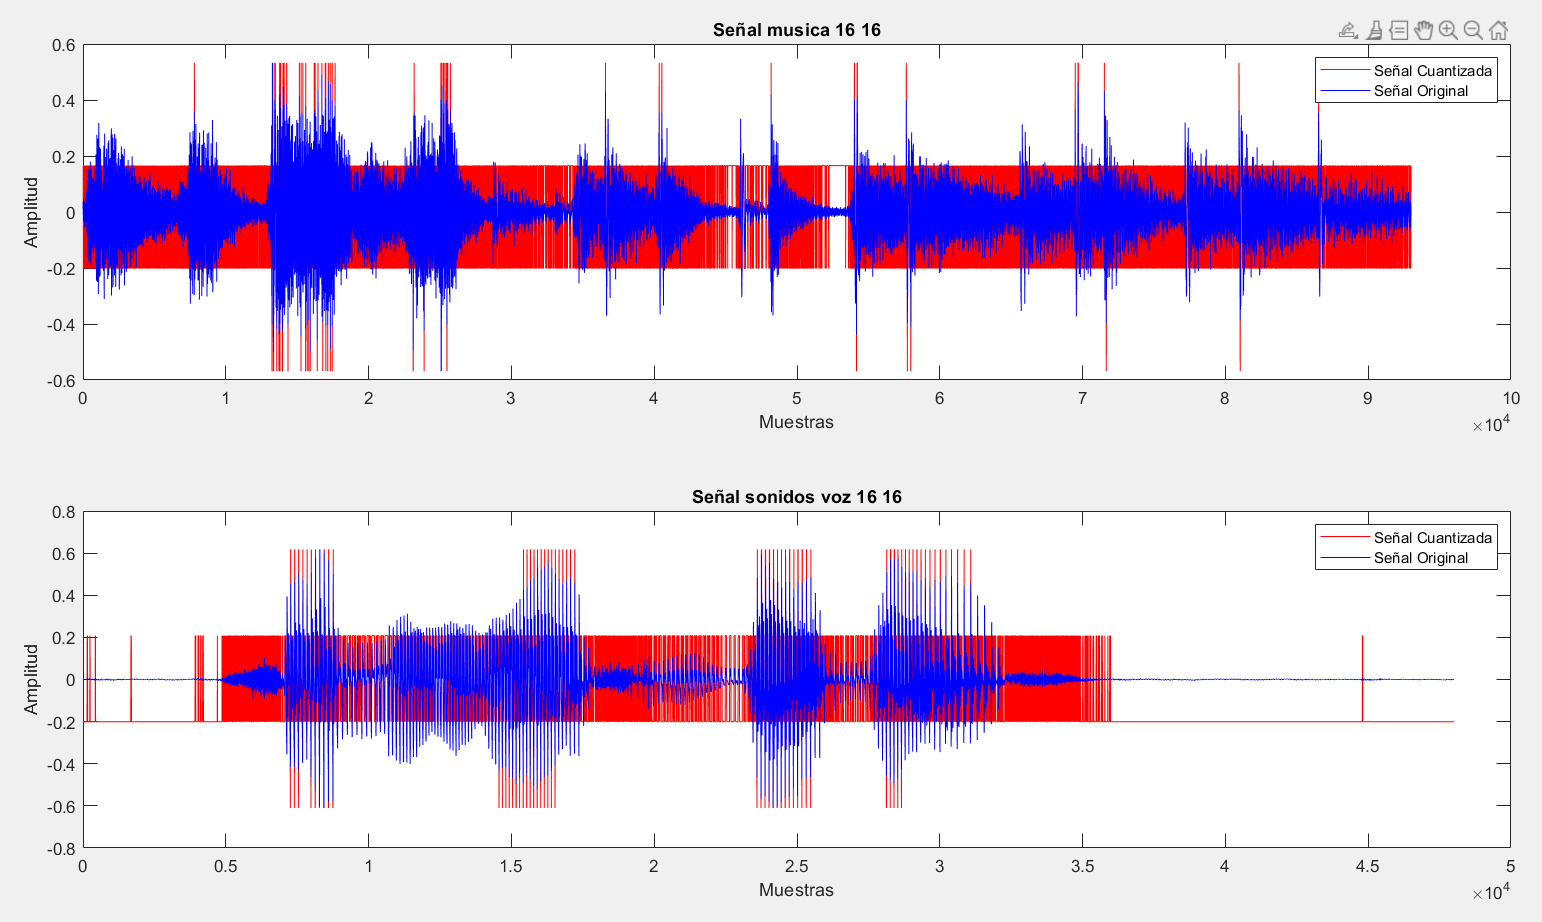
\includegraphics[scale=0.4]{Figuras/plotV2a.png}
        \caption{Señales cuantizadas superpuestas a su señal original.}\label{V2a}
        \end{figure}
        
        \item El histograma obtenido para 2 bits de cuantización se muestra en la Figura \ref{V2b}.
        Comparando los histogramas para los diferentes niveles de cuantización notamos que con más bits de cuantización el histograma toma una forma uniforme y a medida que disminuimos estos bits, la frecuencia de error en torno a cero disminuye ya que el error respecto a la señal cuantizada y la original en cada muestra es más frecuente.
        
        \begin{figure}[H]
        \centering
        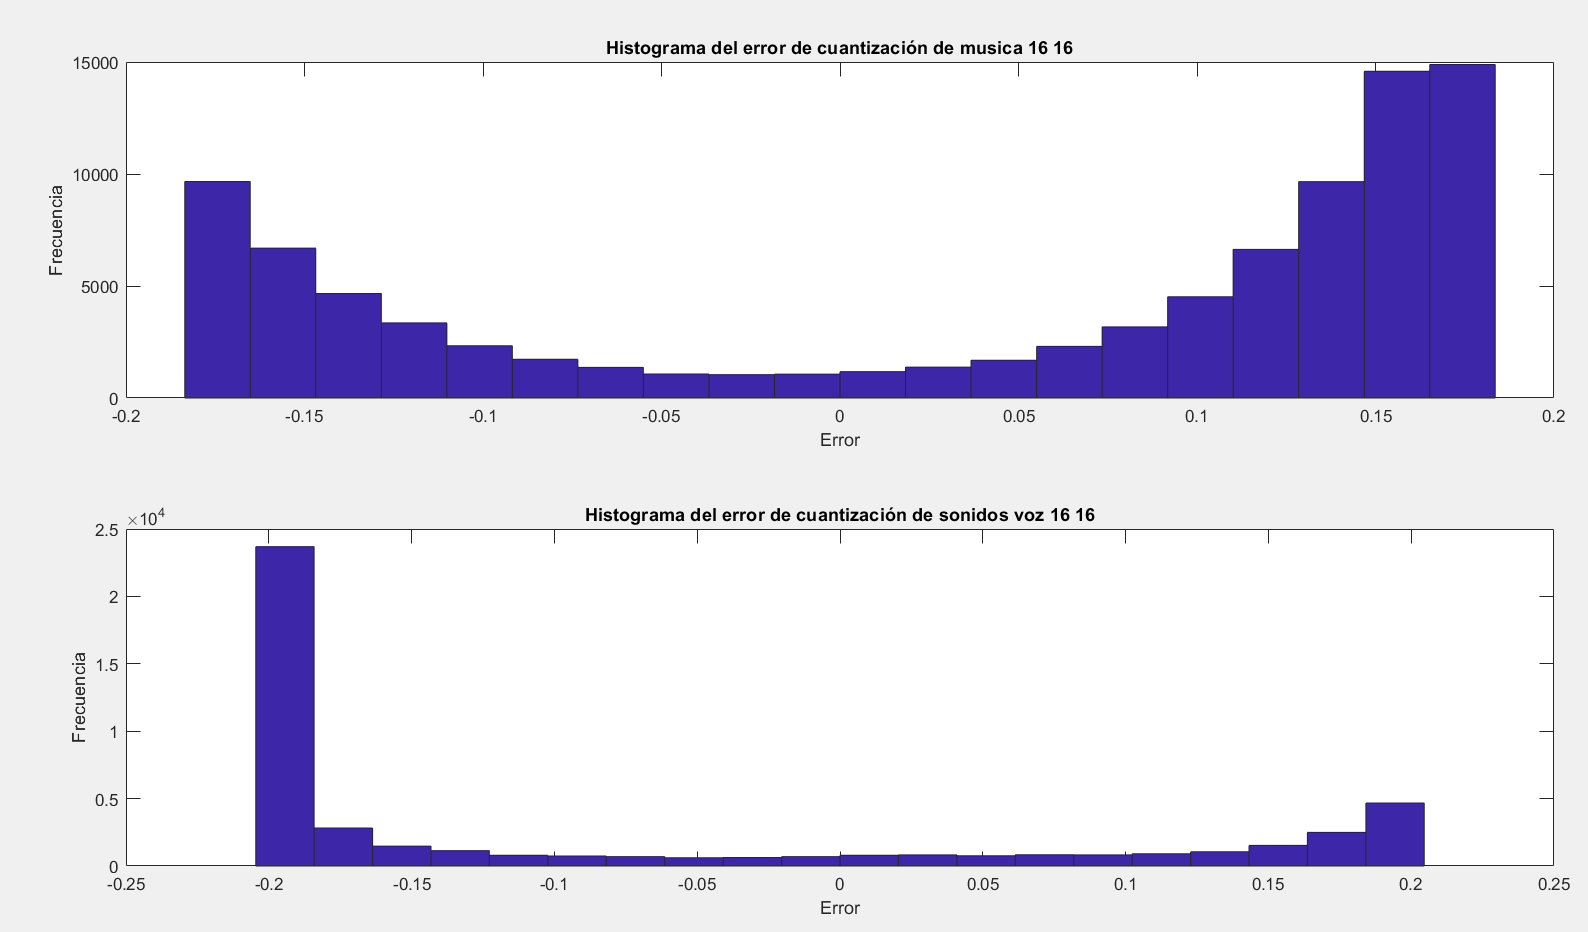
\includegraphics[scale=0.4]{Figuras/plotV2b.png}
        \caption{Histograma de error de cuantización.}\label{V2b}
        \end{figure}
        
        \item 
        \begin{itemize}
        \item
        Se obtuvieron señales para la correlación entre la señal y el error y la autocorrelación del error para $n=2$ y $n=12$. Los gráficos obtenidos se presentan en la figuras \ref{VC2} y \ref{VC12}.
        \item 
        La reducción de bits aumenta mucho la correlación entre la señal cuantizada y el ruido de cuantización. En la figura \ref{VC2} se observa que esta tiene peaks en 0, los cuales desaparecen completamente al aumentar la tasa a 12 bits.
        
        La autocorrelación del ruido siempre conserva su peak en 0 (lo cual tiene sentido al estar calculando una correlación), pero su autocorrelación ante otros puntos disminuye completamente al aumentar la cantidad de niveles de cuantización.
        \item
        El número de niveles de cuantización afecta a la correlación, haciendo que esta disminuya cuando $n$ aumenta. Lo cual también es consistente con la aproximación del error a una variable uniforme al aumentar los niveles de cuantización.
        \end{itemize}
        \begin{figure}[H]
            \centering
            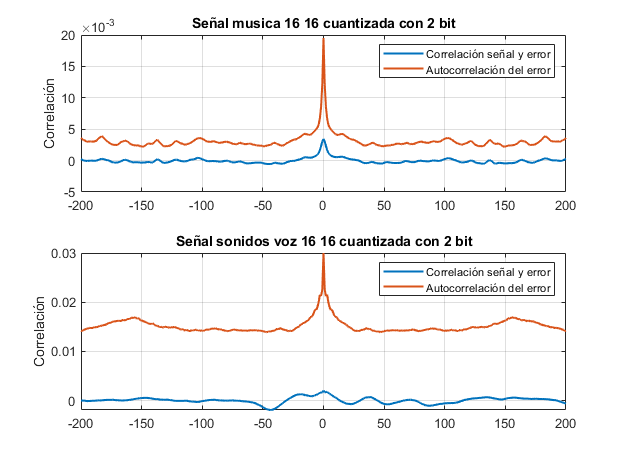
\includegraphics[width=0.7 \linewidth]{Figuras/PLOTVC2.png}
            \caption{Correlaciónes entre ruido y señal para n=2}
            \label{VC2}
        \end{figure}
        \begin{figure}[H]
            \centering
            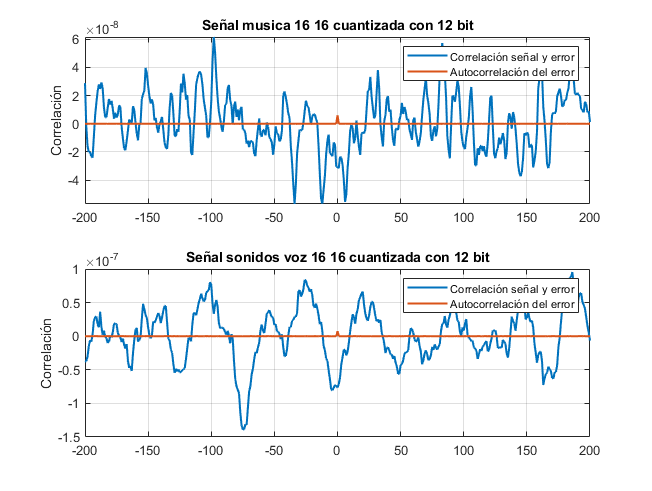
\includegraphics[width=0.7 \linewidth]{Figuras/PLOTVC12.png}
            \caption{Correlaciónes entre ruido y señal para n=12}
            \label{VC12}
        \end{figure}
    \end{enumerate}
    \item El codigo implementado para la función $cuantiza\_dither$ se presenta a continuación:
    
     \begin{lstlisting}[frame=single]
    function c = cuantiza_dither(x,N)
    delta = (max(x)-min(x))/(N-1);
    W = (delta*0.25).*randn(length(x),1);
    J = x + W;
    deltaJ = (max(J)-min(J))/(N-1);
    S1 =  (J-min(J))/deltaJ;
    c = round(S1);
    end
    \end{lstlisting}
    
    Si bien se mantiene la presencia de ruido tanto en las señales con o sin dither, para la señal con dithering se percibe un ruido general de fondo, que se mantiene similar sin importar la intensidad de la señal de audio, lo que permite que esta se oiga más clara. Para el otro caso, se escucha un ruido que sigue y "distorsiona" la señal original, dificultando la escucha de ella.
    
    El dither cumple la función de eliminar la correlación entre señal y ruido de cuantización, lo que podría facilitar técnicas de filtrado para recuperar la señal original.
    
\end{enumerate}

%%%%%%%%%%%%%%%%%%%%%%%%%%%%%%%%%%%%%%%%%%%%%%%%%%%%%%%%%%%%%%%%%%%%%%%%%%%%%%%%%%%%%%%%%%%%%%%%%%
%
%----------------------------------OPERACI ́ON B ́ASICA CON PUNTO FIOS----------------------------%
%
%%%%%%%%%%%%%%%%%%%%%%%%%%%%%%%%%%%%%%%%%%%%%%%%%%%%%%%%%%%%%%%%%%%%%%%%%%%%%%%%%%%%%%%%%%%%%%%%%%
\section{Operación básica con punto fijo}

\begin{enumerate}[{a)}]
    \item 
    \begin{itemize}
        \item 
        Al estar trabajando con números enteros de 16 bytes (variables de tipo \texttt{int16}), conviene usar todos los valores disponibles para la creación de la ventana $w$, es decir generar una ventana con numeros que van desde $0$ a $2^{15}$. Si consideramos estos numeros mediante representación Q15, la ventana iría entre $0$ y $1$. \\
        Utilizando el comando \texttt{whos(w)} y \texttt{whos(h)}, siendo $h$ la ventana creada directamente usando \texttt{blackman()}, se observa que $w$ ocupa 322 bytes, mientras que $h$ utiliza 1288 bytes. Lo que comprueba que las variables \textit{int16} utilizan cuatro veces menos espacio que las de tipo \textit{double}.
        \item
        Se creo la señal enventanada $y$ con el siguiente código:
        \begin{lstlisting}
        [dataVI,fs]=audioread("aliasing_test_16_16.wav", 'native');
        N=int16(161);
        x=dataVI(1:N);
        ww=blackman(N)*2^15;
        w=int16(ww);
        y=int32(w).*int32(x);
        y=int16(y*2^(-15));
        \end{lstlisting}
        Cabe destacar que al multiplicar dos señales de 16 bits, se deben usar enteros de 32 bits y aplicar el factor de corrección $2^{15}$ antes de volver a los 16 bits.
        Nuevamente $y$ requiere 322 bytes, mientras que cuando se importa con audioread se utilizan 1288 bytes.
        \item
        La figura \ref{VI} muestra las señales obtenidas luego del enventanamiento con operaciones en punto fijo. Cabe notar que en este caso la amplitud de las señales se debe a que MATLAB toma automáticamente los números binarios como complemento 2. Sin embargo, esto no afecta la operatoria si decidimos trabajar en distintas notaciones como Q15 y operar en punto fijo.
        \begin{figure}[H]
            \centering
            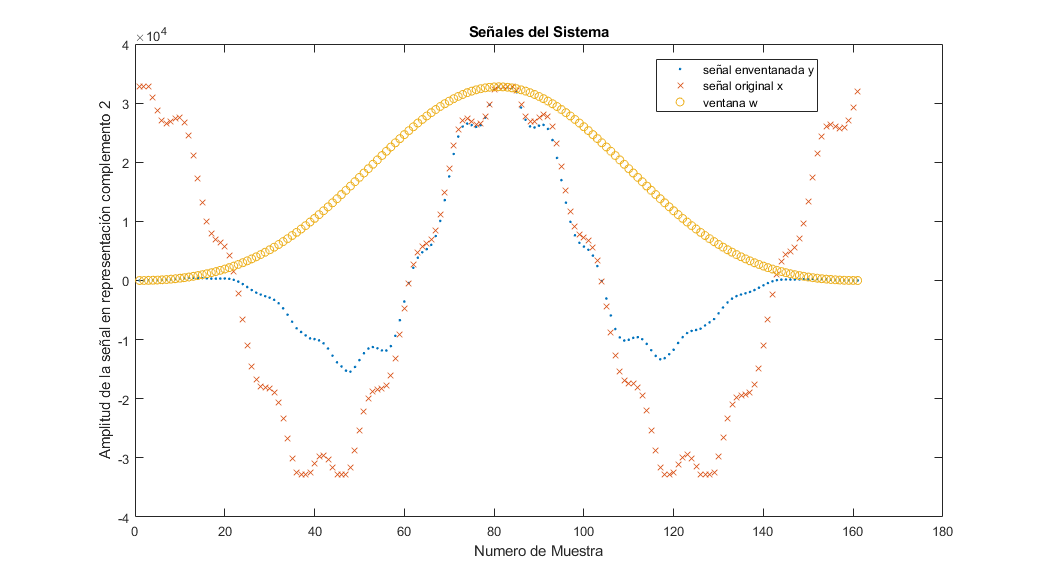
\includegraphics[width= 0.8\linewidth]{Figuras/plotVI.png}
            \caption{Señal original, señal de ventana}
            \label{VI}
        \end{figure}
    \end{itemize}
\end{enumerate}



\end{document}
